\documentclass[10 pt,usenames,dvipsnames, oneside]{article}
\usepackage{../../../modelo-ensino-medio}



\begin{document}

\begin{center}
  \begin{minipage}[l]{3cm}

\includegraphics[width=2cm]{logo}    
\end{minipage}\hfill
\begin{minipage}[r]{.8\textwidth}
 {\Large \scshape Atividade: "Abraçando"{} um círculo com uma reta}  
\end{minipage}
\end{center}
\vspace{.2cm}

\ifdefined\prof
%Habilidades da BNCC
% \begin{objetivos}
% \item 
% \end{objetivos}

%Caixa do Para o Professor
\begin{goals}
%Objetivos específicos
\begin{enumerate}
\item Construir, mais abstratamente em relação à atividade anterior, a sobrejeção da reta sobre a circunferência unitária dada pela função de Euler.
\end{enumerate}

\tcblower

%Orientações e sugestões
Repare que, por enquanto, não estamos preocupados com o sistema de coordenadas do plano que contém a circunferência. Estas coordenadas serão consideradas na próxima seção para formalizar o conceito de seno e cosseno de um número real. Neste momento, o importante é o aluno perceber como fica a posição dos números reais sobre a circunferência unitária após o “enrolar”{} da reta sobre a circunferência.
\end{goals}

\bigskip
\begin{center}
{\large \scshape Atividade}
\end{center}
\fi

Observe a imagem a seguir e responda às perguntas:
\begin{figure}[H]
\centering

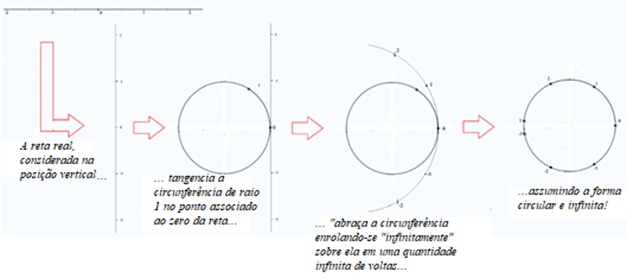
\includegraphics[width=.9\linewidth]{trigonometricas48}
\end{figure}

\begin{enumerate}
\item Quantos pontos da circunferência estarão “cobertos”{} pelo número real $1$?
\item A cada ponto da circunferência, quantos números reais ficam associados?
\item Considerando o ponto $A$ na circunferência sobre o qual encontra-se o número real $1$. Qual o próximo número real positivo que também estará localizado em $A$? E qual será o primeiro número negativo associado a $A$?
\item Se reproduzimos a construção exibida acima usando, em lugar da reta real, o intervalo $[-5,5]$ em uma circunferência de raio $2$, tangenciando esta circunferência no ponto $0$ do intervalo, qual será a medida do menor arco encontrado entre os pontos da circunferência associados a $-5$ e $5$?
\end{enumerate}

\ifdefined\prof
\begin{solucao}

\begin{enumerate}
\item Apenas um ponto ficará coberto por cada número real.
\item A cada ponto da circunferência estarão associados infinitos números reais.
\item A cada arco de volta inteira descrito a partir do ponto $A$ teremos outros pontos da reta que irão se sobrepor em $A$, logo, esses pontos correspondem aos números reais $1 + 2k\pi$, onde que $k$ é um inteiro qualquer. Portanto, o primeiro número positivo após o $1$ cuja posição após o enrolar da reta será o mesmo ponto $A$ é $1 + 2\pi$, enquanto o primeiro número negativo a ser associado a $A$ será $1 - 2\pi$.
\item O ponto em que o número real $5$ está alocado encontra-se no 4º quadrante, visto que está entre $\frac{3\pi}{2}$ e $2\pi$; analogamente, o real $-5$ está no $1$\super{o} quadrante. O menor arco tem comprimento igual a $2\cdot|2\pi-5|$ o que equivale a, aproximadamente, $2{,}5$ unidades de comprimento. Outra maneira de se chegar ao resultado é percebendo que o comprimento do intervalo $[-5,5]$ é $10$, portanto, menor que o comprimento da circunferência de raio $2$, que é $4\pi$ . Portanto, a transformação que enrola o intervalo na circunferência determinará um arco de $10$ unidades e o arco complementar medirá $4\pi − 10$

\begin{figure}[H]
\centering

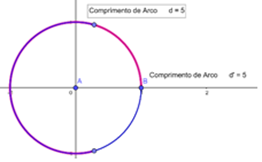
\includegraphics[width=.5\linewidth]{trigonometricas49}
\end{figure}
\end{enumerate}

\end{solucao}
\fi

\end{document}